\section{Результаты эксперимента и обработка данных}
Результат измерений спектра представлен на рис. \ref{spectre_general}. 
При температурах менее 200 К хорошо видно два пика, соответствующих тонкому 
расщеплению верхнего уровня (левый пик -- переходы C и D, правый пик -- переходы
A и B на рис. \ref{Energy levels}). Ясно, что заселённость верхнего уровня
ниже, чем заселённость нижнего, поэтому левый пик обладает большей интенсивностью.
При температурах более 200 К эти два пика перестают быть различимыми. В любом случае
эти пики (или один пик при больших температурах) аппроксимируется лоренцевским
контуром. Исследуются зависимости ширины профиля на полувысоте и положения максимума
от температуры.  

Основные вклады в погрешность вносят неточность измерения температуры и неточность
измерения длины волны. Во-первых, охлаждение при помощи жидкого азота проводилось
очень быстро, поэтому скорости "обновления показателей" термометра не хватало
для точного определения температуры в данный момент времени. К примеру, показания
термометра могли измениться за "один кадр" на более чем 2 градуса. Во-вторых,
используемый спектрометр измеряет интенсивность с шагом $0.1 \text{ нм}$, а ширина
пика составляет $\sim 1 \text{ нм}$, то есть в исследуемой области находится примерно
30 точек на 2 пика. Последнее обстоятельство усугубляется тем, что слева в спектре 
имеются ещё дополнительные переходы на другие колебательные уровни, которые, конечно,
подавлены по сравнению с основными переходами, но существенно ограничивают область,
в которой есть возможность аппроксимировать пик лоренцианом.  

\begin{figure}[!h]
    \begin{center}
        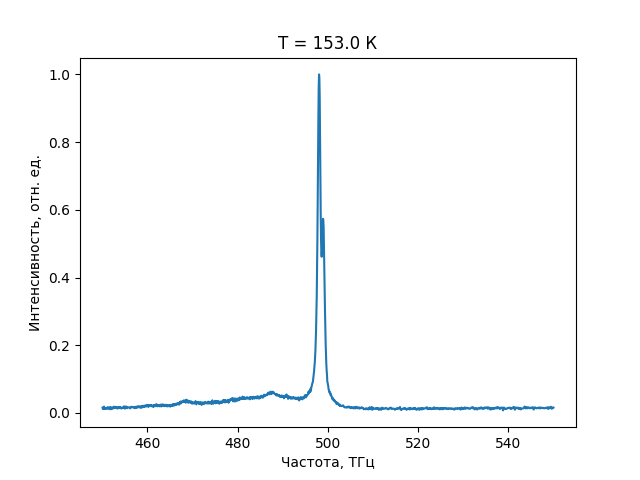
\includegraphics[width=0.7 \linewidth]{spectre_general.png}
        \caption{Спектр люминесценции при температуре T = 153 К.}
        \label{spectre_general}
    \end{center}
\end{figure}


\begin{figure}[!h]
    \begin{minipage}[h]{0.49\linewidth}
        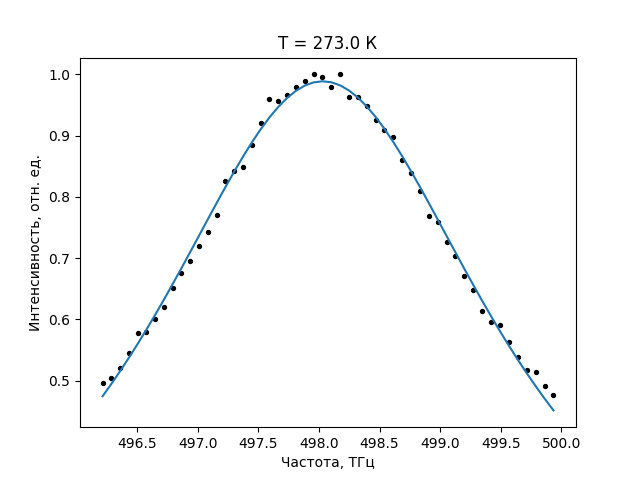
\includegraphics[width = 1.1 \linewidth]{spectre_local_273K.png}
        \\ (a)
    \end{minipage}
    \hfill
    \begin{minipage}[h]{0.49\linewidth}
        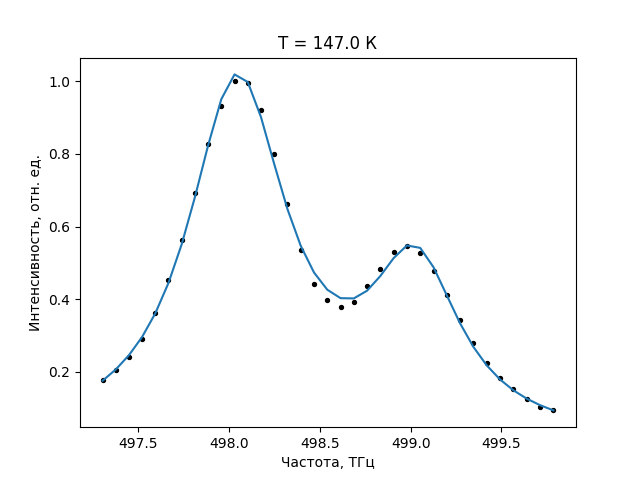
\includegraphics[width = 1.1 \linewidth]{spectre_local_147K.png}
        \\ (a)
    \end{minipage}
    \caption{Аппроксимация лоренцианами пиков спектра люминесценции при температурах
    (a) 273 К, (b) 147 К}
    \label{ris:image1}
\end{figure}